\documentclass{beamer}

\usepackage{comment}
\usepackage{color}
\usepackage{listings}
\usepackage{verbatim}
\usepackage{multicol}
\usepackage{booktabs}
\definecolor{green}{RGB}{0,128,0}

\usetheme{CambridgeUS}
\setbeamercolor*{item}{fg=red}

\def\EQ#1\EN{\begin{equation*}#1\end{equation*}}
\def\BA#1\EA{\begin{align*}#1\end{align*}}
\def\BS#1\ES{\begin{split*}#1\end{split*}}
\newcommand{\bc}{\begin{center}}
\newcommand{\ec}{\end{center}}
\newcommand{\eq}{\ =\ }
\newcommand{\degc}{$^\circ$C}

\def\p{\partial}
\def\qbs{\boldsymbol{q}}
\def\Dbs{\boldsymbol{D}}
\def\A{\mathcal A}
\def\gC{\mathcal C}
\def\gD{\mathcal D}
\def\gL{\mathcal L}
\def\M{\mathcal M}
\def\P{\mathcal P}
\def\Q{\mathcal Q}
\def\gR{\mathcal R}
\def\gS{\mathcal S}
\def\X{\mathcal X}
\def\bnabla{\boldsymbol{\nabla}}
\def\bnu{\boldsymbol{\nu}}
\renewcommand{\a}{{\alpha}}
%\renewcommand{\a}{{}}
\newcommand{\s}{{\sigma}}
\newcommand{\bq}{\boldsymbol{q}}
\newcommand{\bz}{\boldsymbol{z}}
\def\bPsi{\boldsymbol{\Psi}}

\def\Li{\textit{L}}
\def\Fb{\textbf{f}}
\def\Jb{\textbf{J}}
\def\cb{\textbf{c}}

\def\Dt{\Delta t}
\def\tpdt{{t + \Delta t}}
\def\bpsi{\boldsymbol{\psi}}
\def\dbpsi{\delta \boldsymbol{\psi}}
\def\bc{\textbf{c}}
\def\dbc{\delta \textbf{c}}
\def\arrows{\rightleftharpoons}

\newcommand{\bGamma}{\boldsymbol{\Gamma}}
\newcommand{\bOmega}{\boldsymbol{\Omega}}
%\newcommand{\bPsi}{\boldsymbol{\Psi}}
%\newcommand{\bpsi}{\boldsymbol{\psi}}
\newcommand{\bO}{\boldsymbol{O}}
%\newcommand{\bnu}{\boldsymbol{\nu}}
\newcommand{\bdS}{\boldsymbol{dS}}
\newcommand{\bg}{\boldsymbol{g}}
\newcommand{\bk}{\boldsymbol{k}}
%\newcommand{\bq}{\boldsymbol{q}}
\newcommand{\br}{\boldsymbol{r}}
\newcommand{\bR}{\boldsymbol{R}}
\newcommand{\bS}{\boldsymbol{S}}
\newcommand{\bu}{\boldsymbol{u}}
\newcommand{\bv}{\boldsymbol{v}}
%\newcommand{\bz}{\boldsymbol{z}}
\newcommand{\pressure}{P}

\def\water{H$_2$O}
\def\calcium{Ca$^{2+}$}
\def\copper{Cu$^{2+}$}
\def\magnesium{Mg$^{2+}$}
\def\sodium{Na$^+$}
\def\potassium{K$^+$}
\def\uranium{UO$_2^{2+}$}
\def\hion{H$^+$}
\def\bicarbonate{HCO$_3^-$}
\def\cotwo{CO$_2$}
\def\chloride{Cl$^-$}
\def\fluoride{F$^-$}
\def\phosphoricacid{HPO$_4^{2-}$}
\def\nitrate{NO$_3^-$}
\def\sulfate{SO$_4^{2-}$}
\def\souotwooh{$>$SOUO$_2$OH}
\def\sohuotwocothree{$>$SOHUO$_2$CO$_3$}
\def\soh{$>$SOH}

\newcommand\gehcomment[1]{{{\color{orange} #1}}}
\newcommand\add[1]{{{\color{blue} #1}}}
\newcommand\remove[1]{\sout{{\color{red} #1}}}
\newcommand\codecomment[1]{{{\color{green} #1}}}
\newcommand\redcomment[1]{{{\color{red} #1}}}
\newcommand\bluecomment[1]{{{\color{blue} #1}}}
\newcommand\greencomment[1]{{{\color{green} #1}}}

\begin{comment}
\tiny
\scriptsize
\footnotesize
\small
\normalsize
\large
\Large
\LARGE
\huge
\Huge
\end{comment}

\begin{document}
\title{PFLOTRAN Input Cards}
\author{Glenn Hammond}
\date{\today}

\frame{\titlepage}


\subsection{Syntax}

\begin{frame}[fragile,containsverbatim]\frametitle{Syntax}

The PFLOTRAN input deck is defined using keywords or cards that are associated with data.  The file is designed with modularity in mind and the cards need not be in any particular order.  Many cards open a section that provides additional cards and is terminated by an ``END'' or ``/''.  For example:

\begin{semiverbatim}
CARD1
  CARD2 value value
  CARD3
    CARD4 value
    CARD5 value
  /
END
\end{semiverbatim}

\end{frame}

\begin{frame}[fragile]\frametitle{Syntax: Commenting}
Several options exist for commenting out lines or sections of the input file:
\begin{itemize}
\item Individual lines may be commented out by placing a hash (\#) or exclamation point (!) at the beginning of line (i.e. before any text).
\item The SKIP/NOSKIP cards may be used to comment out a large number of lines.  SKIP/NOSKIP may be used in a nested manner.  
\item Comment characters (\# and !) may be used to place comments at the end of a line or to comment out the remainder of a line.
\end{itemize}

\end{frame}

\begin{frame}[containsverbatim]\frametitle{Syntax: Commenting Example}

\begin{semiverbatim}
CARD0
SKIP
CARD1
  ! comment on CARD2
  CARD2 value1 value2
  CARD3
  !  CARD4 value3 
    CARD5 value4 # comment explaining value3
  /
  CARD6 value5 ! comment explaining value5
#  CARD7 value6
  CARD7 value7
END
NOSKIP
CARD8
\end{semiverbatim}

\end{frame}


\documentclass{beamer}

\usepackage{comment}
\usepackage{color}
\usepackage{tabbing}

\title{Types of PFLOTRAN Boundary Conditions\\ Basic}
\author{Glenn Hammond}
\date{\today}

\begin{document}

\frame{\titlepage}

%-----------------------------------------------------------------------------
\section{Flow}
\subsection{Types of Flow Conditions}

\begin{frame}[fragile,containsverbatim]\frametitle{Types of Flow Conditions}

\vspace{0.1in}
\centering
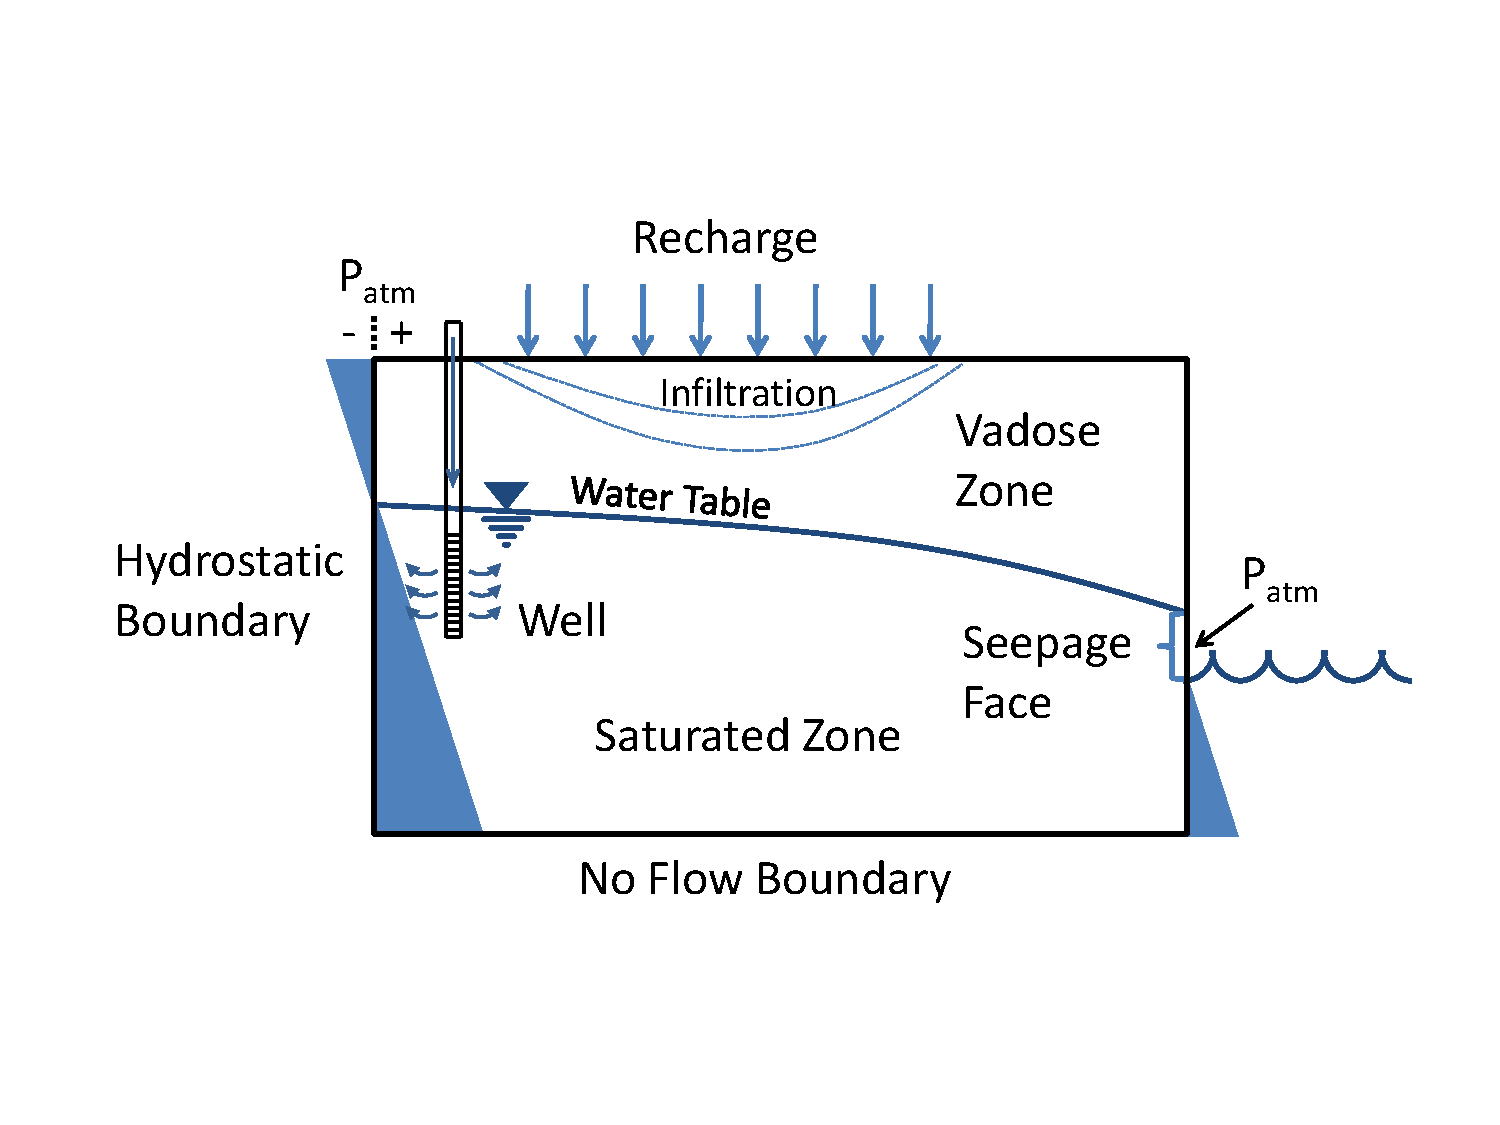
\includegraphics[width=0.9\linewidth]{./flow_bcs_with_well}
%\vspace{-0.5in}
\small 
\begin{tabbing}
\verb|DIRICHLET        |	\= Specified pressure across region\\
\verb|HYDROSTATIC|	      \> Hydrostatic pressure profile across region\\
\verb|SEEPAGE|	         	\> Hydrostatic with outflow only above water table\\
\verb|NEUMANN|			      \> Darcy flux across boundary [L/T]\\
\verb|MASS_RATE|	      	\> Mass injection/extraction rate [M/T]\\
\verb|VOLUMETRIC_RATE|	  \> Volumetric injection/extraction rate [L$^3$/T]\\
\end{tabbing}

\end{frame}


\section{Transport}
\subsection{Types of Transport Conditions}

\begin{frame}[fragile,containsverbatim]\frametitle{Types of Transport Conditions}

\vspace{0.1in}
\centering
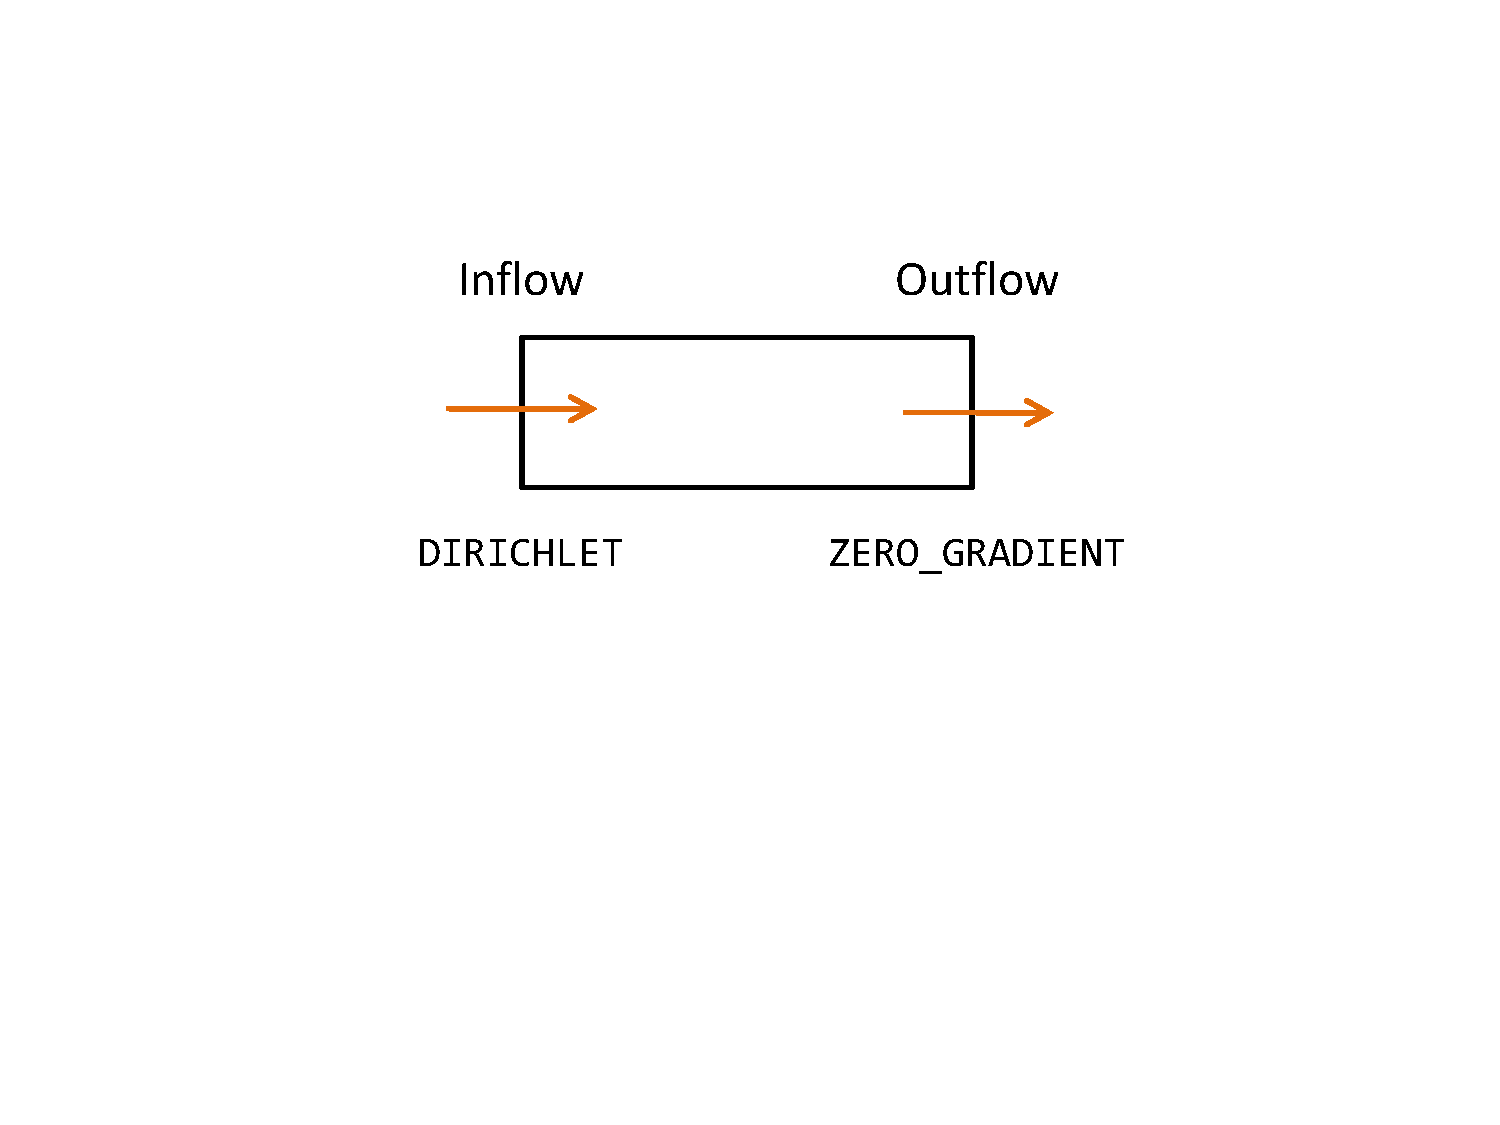
\includegraphics[width=0.5\linewidth]{./transport_bcs_unidirectional}
\vspace{0.1in}
\hline
\vspace{0.1in}
\hspace{-6mm}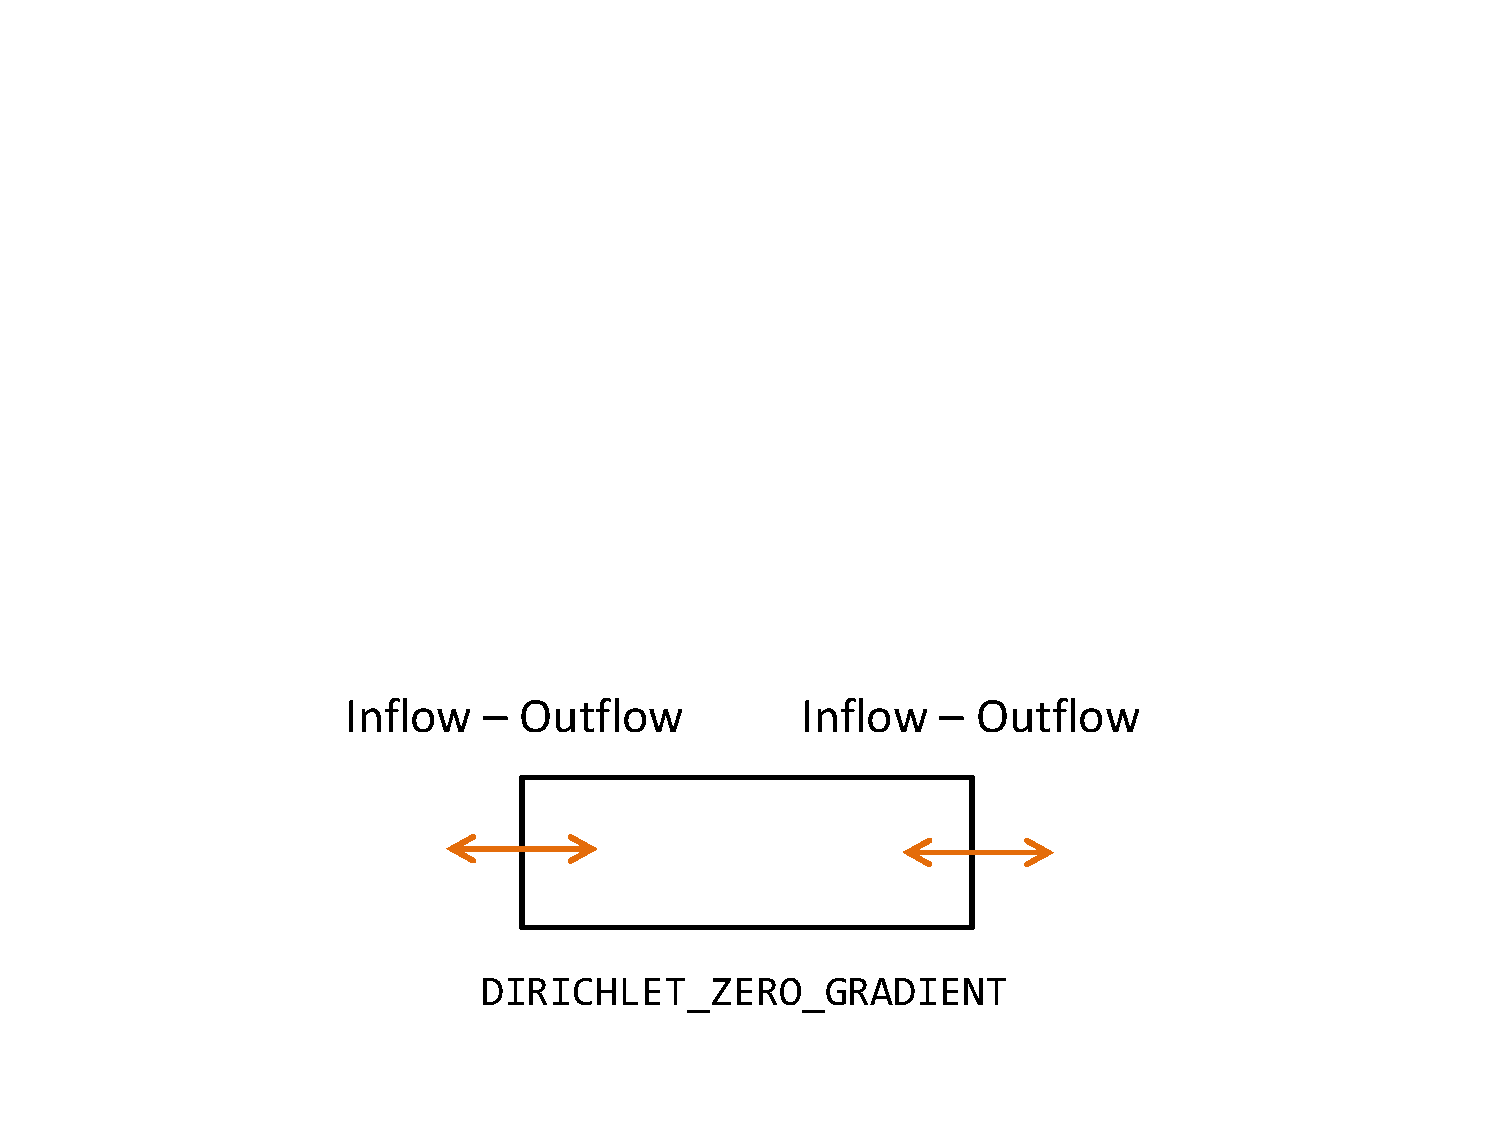
\includegraphics[width=0.58\linewidth]{./transport_bcs_bidirectional}

\begin{tabbing}
\verb|DIRICHLET                 |	\= Specified concentration\\
\verb|ZERO_GRADIENT|     	        \> Zero diffusive flux\\
\verb|DIRICHLET_ZERO_GRADIENT|		\> Hybrid for inflow - outflow
\end{tabbing}

\end{frame}




\end{document}
\section{CHECKPOINT Card}

\begin{frame}[fragile,containsverbatim]\frametitle{CHECKPOINT}

\begin{itemize}{}
\item[] \textbf{Purpose:} Toggle on checkpoint/restart capability and specifies the frequency at which checkpoint files are created.  A restart file is created when the simulation terminates as scheduled.

\item[] \textbf{Example uses:}
\begin{itemize}
\item Save the state of a simulation every 100 time steps
\item Save the state of a simulation once the final time has been reached.  
\item Fault tolerance
\end{itemize}
\end{itemize}

\end{frame}



\subsection{CHEMISTRY}

\begin{frame}[fragile,containsverbatim]\frametitle{CHEMISTRY}

\begin{itemize}
\item[] \textbf{Purpose:} Define aqueous chemistry for problem
\item[] \textbf{Example uses:}
\begin{itemize}
  \item Conservative solute transport
  \item Multicomponet biogeochemical transport
\end{itemize}
\item[] \textbf{Key sub-cards:}
\begin{itemize}
  \item[] \verb|PRIMARY_SPECIES|
  \item[] \verb|SECONDARY_SPECIES|
  \item[] \verb|IMMOBILE_SPECIES|
  \item[] \verb|MINERALS|
  \item[] \verb|MINERAL_KINETICS|
  \item[] \verb|SORPTION|
  \item[] \verb|ACTIVITY_COEFFICIENTS|
  \item[] \verb|RADIOACTIVE_DECAY_REACTION|
  
\end{itemize}
\end{itemize}

\end{frame}

%-----------------------------------------------------------------------------
\begin{frame}[fragile]\frametitle{CHEMISTRY Example: Solute Transport}

\begin{semiverbatim}
CHEMISTRY
  PRIMARY_SPECIES
    Tracer
    Tracer2
  /
  OUTPUT
    TOTAL
    ALL
  /
END
\end{semiverbatim}

\end{frame}

%-----------------------------------------------------------------------------
\begin{frame}[fragile]\frametitle{CHEMISTRY Example: Carbonate Chemistry}

\tiny
\begin{semiverbatim}
CHEMISTRY
  PRIMARY_SPECIES
    H+
    HCO3-
    Ca++
  /
  SECONDARY_SPECIES
    OH-
    CO3--
    CO2(aq)
    CaCO3(aq)
    CaHCO3+
    CaOH+
  /
  GAS_SPECIES
    CO2(g)
  /
  MINERALS
    Calcite
  /
  MINERAL_KINETICS
    Calcite
      RATE_CONSTANT 1.d-6 mol/m^2-sec
    /
  /
  DATABASE ../../../database/hanford.dat
  LOG_FORMULATION
  ACTIVITY_COEFFICIENTS TIMESTEP
  OUTPUT
    PH
    TOTAL
    ALL
  /
END
\end{semiverbatim}

\end{frame}

\subsection{CONSTRAINT}

\begin{frame}[fragile,containsverbatim]\frametitle{CONSTRAINT}

\begin{itemize}
\item[] \textbf{Purpose:} A snapshot of chemistry
\item[] \textbf{Example uses:}
\begin{itemize}
  \item Defining aqueous chemistry
  \item Defining mineralogy
\end{itemize}
\item[] \textbf{Key sub-cards:}
\begin{itemize}
  \item[] \verb|CONCENTRATIONS|
  \item[] \verb|SURFACE_COMPLEXES|
  \item[] \verb|IMMOBILE|
  \item[] \verb|MINERALS|
\end{itemize}
\end{itemize}

\end{frame}

%-----------------------------------------------------------------------------
\begin{frame}[fragile]\frametitle{CONSTRAINT Example: Solutes}

\begin{semiverbatim}
CONSTRAINT initial
  CONCENTRATIONS
    Tracer  1.d-10 T
    Tracer2 1.d-10 T
  /
END
\end{semiverbatim}

\end{frame}

%-----------------------------------------------------------------------------
\begin{frame}[fragile]\frametitle{CONSTRAINT Example: Carbonate Chemistry}

\begin{semiverbatim}
CONSTRAINT equilibrated
  CONCENTRATIONS
    H+     1.d-8      F
    HCO3-  1.d-3      G  CO2(g)
    Ca++   5.d-4      M  Calcite
  /
  MINERALS
    Calcite 1.d-5 1.d0 m^2/m^3
  /
END
\end{semiverbatim}

\end{frame}

\section{Coupler}

\begin{frame}[fragile,containsverbatim]\frametitle{PFLOTRAN Coupler}

\begin{itemize}
\item[] \textbf{Purpose:} Couples a flow and/or transport conditions with a region to create a boundary condition, initial condition or source/sink.
\item[] \textbf{Example uses:}
\begin{itemize}
  \item Assign a boundary condition to a face of the model
  \item Assign initial concentrations to a zone in the model
  \item Assign an injection well with in the model domain
\end{itemize}
\end{itemize}
\end{frame}

\begin{frame}[fragile,containsverbatim]\frametitle{PFLOTRAN Coupler}
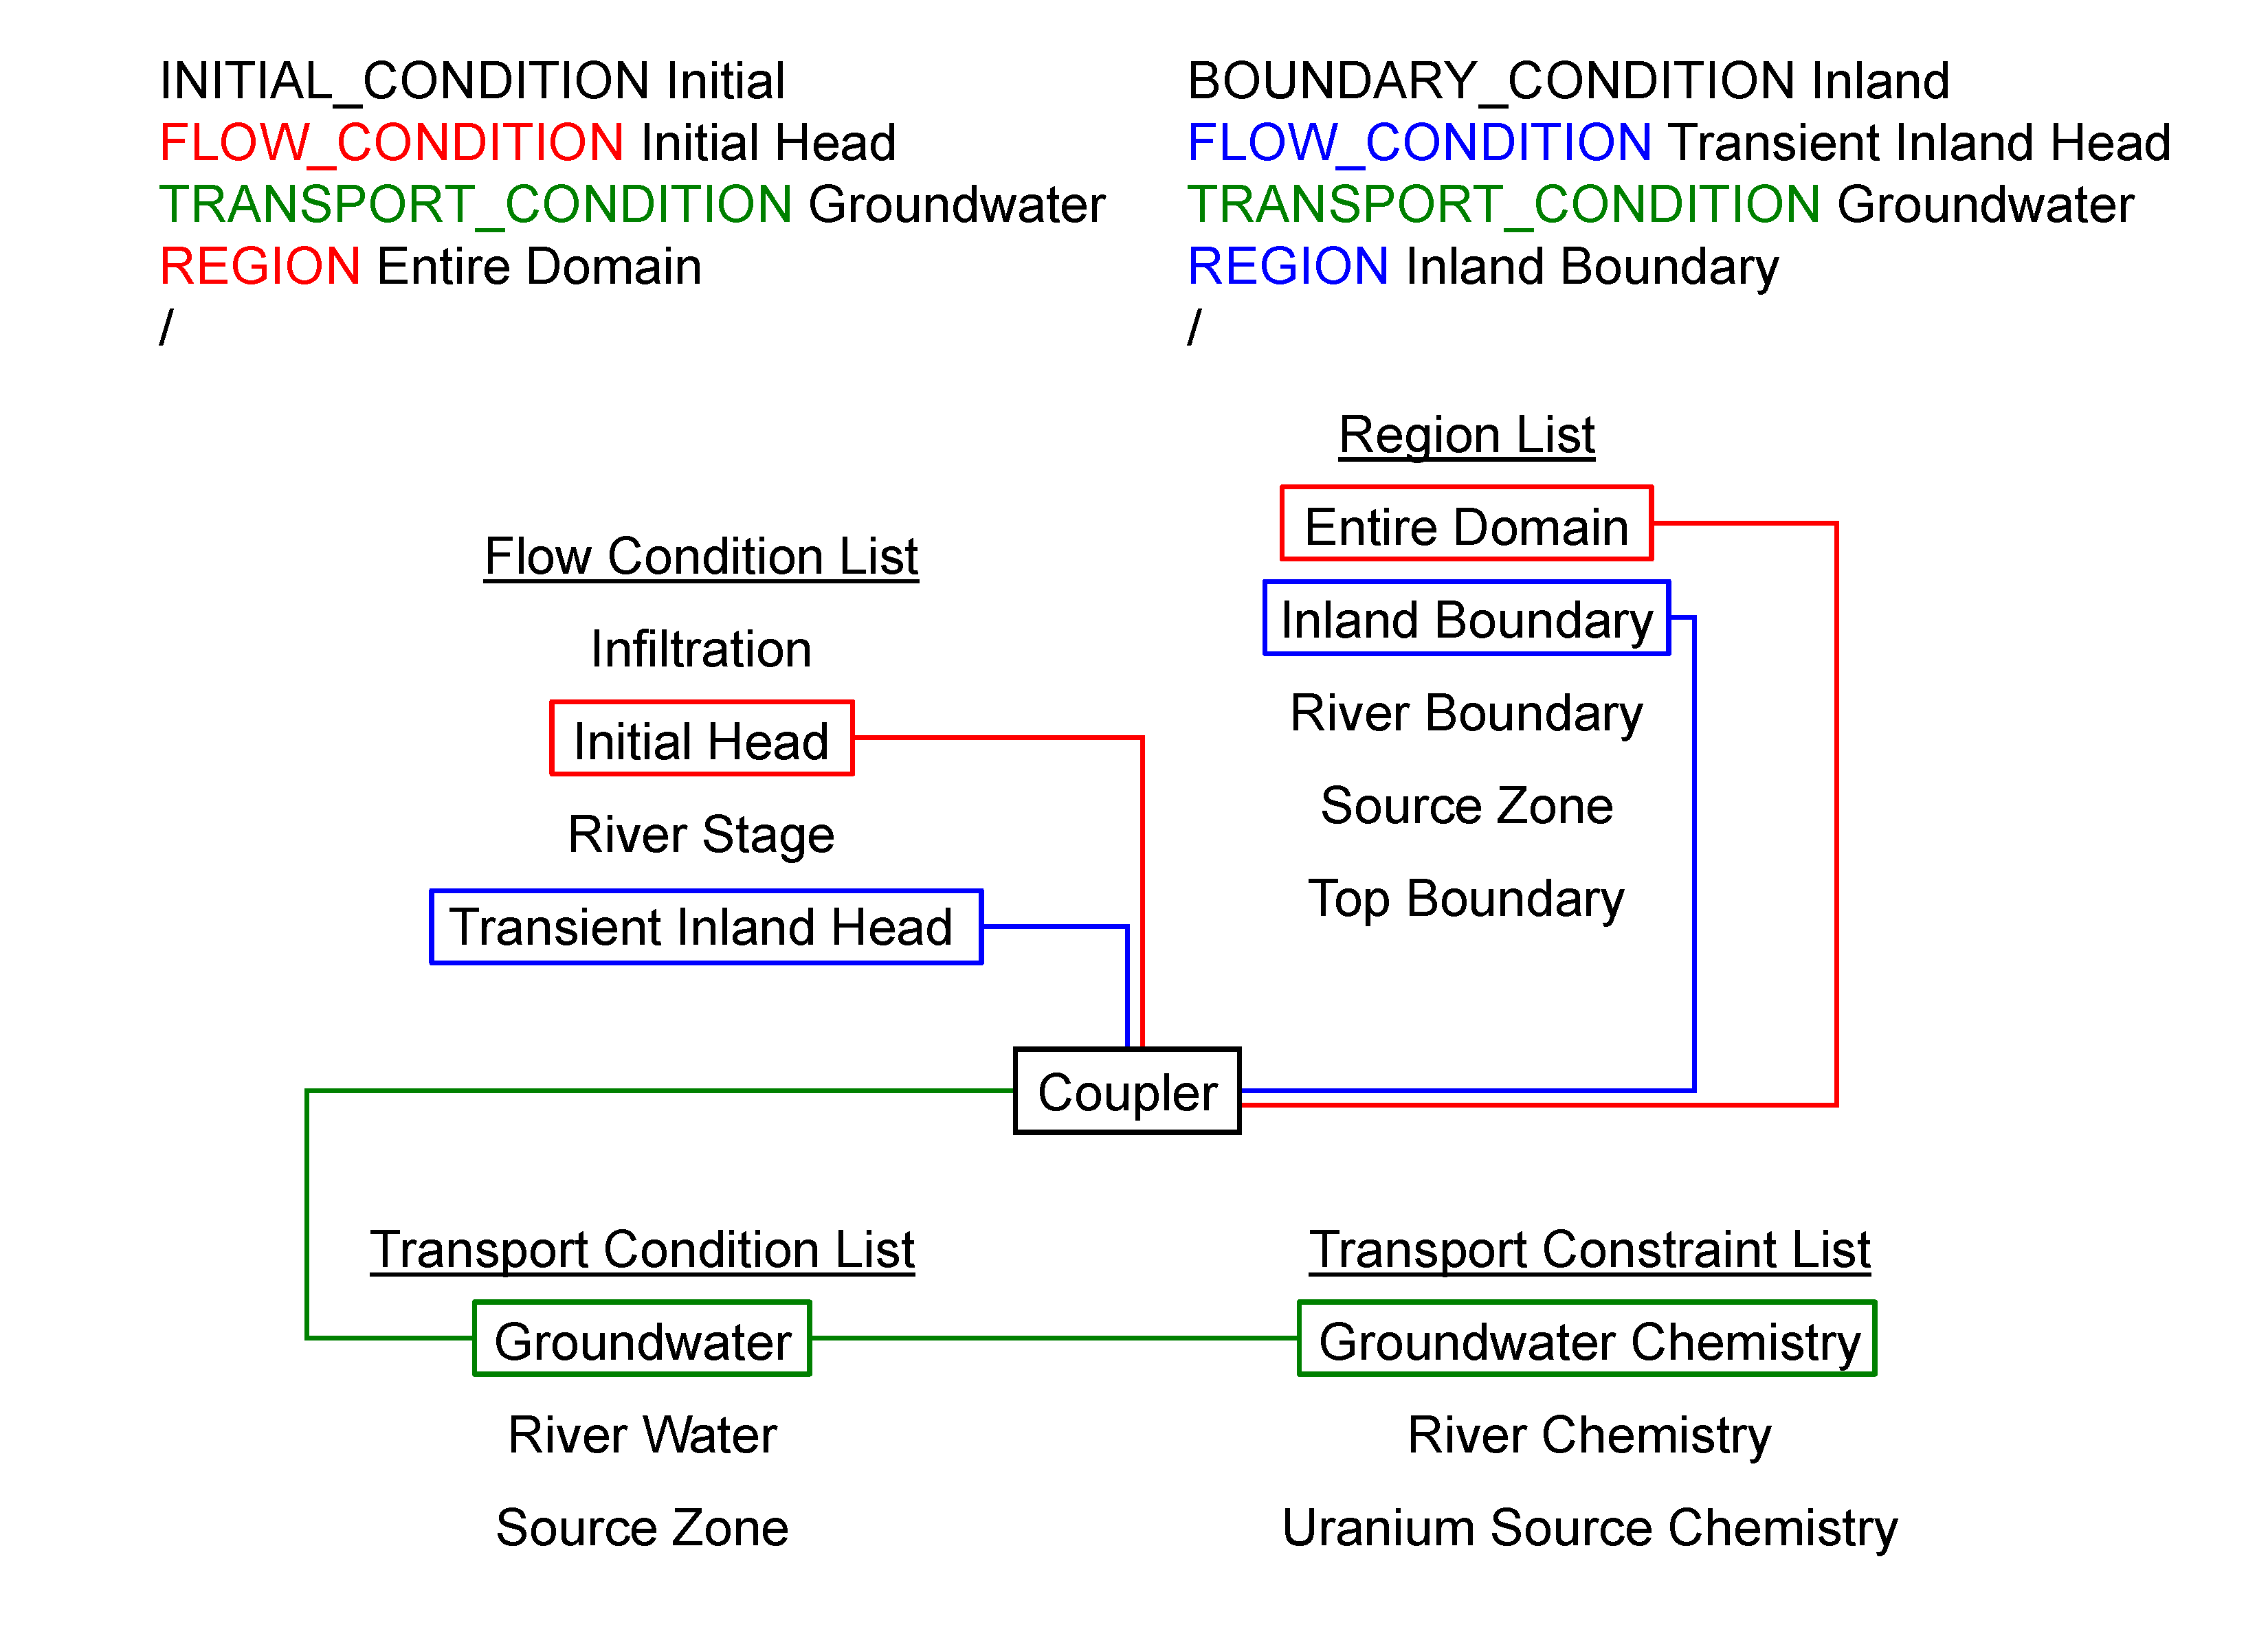
\includegraphics[width=\linewidth]{coupler.pdf}
\end{frame}

[suites]
standard = top_surface_node_centered
           top_surface_cell_centered
           east_surface_node_centered
           east_surface_cell_centered
           north_surface_node_centered
           north_surface_cell_centered
           x_line_node_centered
           x_line_cell_centered
           y_line_node_centered
           y_line_cell_centered
           z_line_node_centered
           z_line_cell_centered
           543_river_het_map_dirich
           543_river_het_map_seep
           543_river_het_map_conduct
standard_parallel = 543_river_het_map_dirich-np4

[default-test-criteria]
# default criteria for all tests, can be overwritten by specific tests
time = 500 percent
generic = 1.0e-12 absolute
concentration = 1.0e-9 relative
discrete = 0 absolute
rate = 1.0e-12 absolute
volume_fraction = 1.0e-12 absolute
pressure = 1.0e-12 relative
saturation = 1.0e-12 absolute

[top_surface_node_centered]

[top_surface_cell_centered]

[east_surface_node_centered]

[east_surface_cell_centered]

[north_surface_node_centered]

[north_surface_cell_centered]

[x_line_node_centered]

[x_line_cell_centered]

[y_line_node_centered]

[y_line_cell_centered]

[z_line_node_centered]

[z_line_cell_centered]

[543_river_het_map_dirich]

[543_river_het_map_dirich-np4]
np=4

[543_river_het_map_seep]

[543_river_het_map_conduct]


\section{DEBUG Card}

\begin{frame}[fragile,containsverbatim]\frametitle{DEBUG}

\begin{itemize}{}
\item[] \textbf{Purpose:} A list of toggles for turning on the writing of vectors and matrices for debugging purposes.

\item[] \textbf{Example uses:}
\begin{itemize}
\item Print the Jacobian
\item Print the residual vector
\end{itemize}
\end{itemize}

\end{frame}



\subsection{FLOW\_CONDITION}

\begin{frame}[fragile,containsverbatim]\frametitle{FLOW\_CONDITION}

\begin{itemize}
\item[] \textbf{Purpose:} Defines parameters/conditions to be associated with flow boundary and initial conditions
\item[] \textbf{Example uses:}
\begin{itemize}
  \item Specify a constant pressures on cell faces
  \item Specify a transient fluxes through cell faces
  \item Define a hydrostatic column of water
\end{itemize}
\item[] \textbf{Key sub-cards:}
\begin{itemize}
  \item[] \verb|TYPE|
  \item[] \verb|  DIRICHLET|
  \item[] \verb|  NEUMANN|
  \item[] \verb|  RATE|
  \item[] \verb|DATUM|
  \item[] \verb|GRADIENT|
  \item[] \verb|PRESSURE|
  \item[] \verb|FLUX|
  \item[] \verb|RATE|
\end{itemize}
\end{itemize}

\end{frame}

%-----------------------------------------------------------------------------
\begin{frame}[fragile]\frametitle{FLOW\_CONDITION Example: Undulating River}

\begin{semiverbatim}
FLOW_CONDITION river
  TYPE
    PRESSURE HYDROSTATIC
  /
  INTERPOLATION LINEAR
  DATUM LIST
    TIME_UNITS d
    0.d0 0.d0 0.d0 34.d0
    10.d0 0.d0 0.d0 39.d0
    50.d0 0.d0 0.d0 33.d0
    100.d0 0.d0 0.d0 34.d0
  /
  PRESSURE 101325 ! Pa
END
\end{semiverbatim}

\end{frame}

%-----------------------------------------------------------------------------
\begin{frame}[fragile]\frametitle{FLOW\_CONDITION Example: Transient Rainfall}

\begin{semiverbatim}
FLOW_CONDITION recharge
  TYPE
    FLUX NEUMANN
  /
  FLUX LIST
    TIME_UNITS yr
    DATA_UNITS cm/yr
    0.d0 25.d0
    1.d0 23.d0
    2.d0 27.d0
    3.d0 22.d0
    4.d0 24.d0
    5.d0 29.d0
  /
END
\end{semiverbatim}

\end{frame}

%-----------------------------------------------------------------------------
\begin{frame}[fragile]\frametitle{FLOW\_CONDITION Example: Permeability-Weighted Injection Well}

\begin{semiverbatim}
FLOW_CONDITION injection_well
  TYPE
    RATE SCALED_VOLUMETRIC_RATE NEIGHBOR_PERM
  /
  RATE 1 m^3/hr
END
\end{semiverbatim}

\end{frame}

\subsection{FLUID\_PROPERTY}

\begin{frame}[fragile,containsverbatim]\frametitle{FLUID\_PROPERTY}

\begin{itemize}
\item[] \textbf{Purpose:} Define fluid properties
\item[] \textbf{Example uses:}
\begin{itemize}
  \item Set coefficient fo molecular diffusion
\end{itemize}
\item[] \textbf{Key sub-cards:}
\begin{itemize}
  \item[] \verb|DIFFUSION_COEFFICIENT|
\end{itemize}
\end{itemize}

\end{frame}

%-----------------------------------------------------------------------------
\begin{frame}[fragile]\frametitle{FLUID\_PROPERTY Example}

\begin{semiverbatim}
FLUID_PROPERTY 
  DIFFUSION_COEFFICIENT 1.d-9
END
\end{semiverbatim}

\end{frame}

\subsection{GRID}

\begin{frame}[fragile,containsverbatim]\frametitle{GRID}

\begin{itemize}
\item[] \textbf{Purpose:} Defines the physically discretized domain
\item[] \textbf{Example uses:}
\begin{itemize}
  \item Type of discretization [structured, unstructured]
  \item Extent of domain
  \item Grid resolution
  \item Specifying direction of gravity vector
\end{itemize}
\item[] \textbf{Key sub-cards:}
\begin{itemize}
  \item[] \verb|TYPE|
  \item[] \verb|  STRUCTURED|
  \item[] \verb|  UNSTRUCTURED|
  \item[] \verb|  UNSTRUCTURED_EXPLICIT|
  \item[] \verb|ORIGIN|
  \item[] \verb|BOUNDS|
  \item[] \verb|NXYZ|
  \item[] \verb|DXYZ|
\end{itemize}
\end{itemize}

\end{frame}

%-----------------------------------------------------------------------------
\begin{frame}[fragile]\frametitle{GRID Example: Cartesian Grid with BOUNDS}

\begin{semiverbatim}
GRID
  TYPE STRUCTURED
  NXYZ 16 16 16
  BOUNDS
    0.d0 0.d0 0.d0
    16.d0 16.d0 16.d0
  /
END
\end{semiverbatim}

\end{frame}

%-----------------------------------------------------------------------------
\begin{frame}[fragile]\frametitle{GRID Example: Cartesian Grid with DXYZ}

\begin{semiverbatim}
GRID
  TYPE STRUCTURED
  ORIGIN 0.d0 0.d0 0.d0
  NXYZ 5 4 3
  DXYZ
    10. 11. 12. 13. 14.
    13. 12. 11. 10.
    15. 20. 25.
  /
END
\end{semiverbatim}

\end{frame}

%-----------------------------------------------------------------------------
\begin{frame}[fragile]\frametitle{GRID Example: Explicit Unstructured Grid}

\begin{semiverbatim}
GRID
  TYPE UNSTRUCTURED_EXPLICIT ./mixed.uge
END
\end{semiverbatim}
\textit{mixed.uge contents}
\begin{semiverbatim}
CELLS 15
1 4.0625 4.0625 4.0625 5.20833
2 4.375 4.375 3.125 2.60417
...
15 1.25 3.75 0.3125 2.60417
CONNECTIONS 24
1 2 4.16667 4.16667 3.3333 6.25
1 3 3.75 3.75 3.75 8.8388
...
14 15 0.41667 3.75 0.41667 2.2097
\end{semiverbatim}

\end{frame}

\section{INITIAL\_CONDITION Card}

\begin{frame}[fragile,containsverbatim]\frametitle{INITIAL\_CONDITION}

\begin{itemize}
\item[] \textbf{Purpose:} Couples a flow and/or transport conditions with a region to create an initial condition.
\item[] \textbf{Example uses:}
\begin{itemize}
  \item To assign a initial condition.
\end{itemize}
\end{itemize}

\end{frame}

\begin{frame}[fragile]\frametitle{INITIAL\_CONDITION: Examples}

\end{frame}

\section{LINEAR\_SOLVER Card}

\begin{frame}[fragile,containsverbatim]\frametitle{LINEAR\_SOLVER}

\begin{itemize}
\item[] \textbf{Purpose:} Defines the linear solver and preconditioner to be employed and linear solver convergence criteria
\item[] \textbf{Example uses:}
\begin{itemize}
  \item Assigning a direct solver (e.g. LU)
  \item Assigning a Krylov solver (e.g. BiCGSTAB)
  \item Assigning a preconditioner (e.g. block Jacobi, ILU[0])
  \item Defining linear solver convergence criteria
  \item Defining pivoting tolerances for LU/ILU
\end{itemize}
\end{itemize}

\end{frame}

\begin{frame}[fragile]\frametitle{LINEAR\_SOLVER: Examples}

\end{frame}

\subsection{MATERIAL\_PROPERTY}

\begin{frame}[fragile,containsverbatim]\frametitle{MATERIAL\_PROPERTY}

\begin{itemize}
\item[] \textbf{Purpose:} Define material properties for simulation.
\item[] \textbf{Example uses:}
\begin{itemize}
  \item Associate ID with material properties
  \item Specify porosity, permeability, rock/soil particle density
  \item Associate constitutive relations (e.g. saturation functions, relative permeability functions)
\end{itemize}
\item[] \textbf{Key sub-cards:}
\begin{itemize}
  \item[] \verb|ID|
  \item[] \verb|POROSITY|
  \item[] \verb|TORTUOSITY|
  \item[] \verb|PERMEABILITY|
  \item[] \verb|ROCK_DENSITY|
  \item[] \verb|SPECIFIC_HEAT|
  \item[] \verb|CHARACTERISTIC_CURVES|
  \item[] \verb|SOIL_COMPRESSIBILITY|
\end{itemize}
\end{itemize}

\end{frame}

%-----------------------------------------------------------------------------
\begin{frame}[fragile]\frametitle{MATERIAL\_PROPERTY Example: Solute Transport}

\begin{semiverbatim}
MATERIAL_PROPERTY soil
  ID 1
  POROSITY 0.25d0
  TORTUOSITY 1.d0
END
\end{semiverbatim}

\end{frame}

%-----------------------------------------------------------------------------
\begin{frame}[fragile]\frametitle{MATERIAL\_PROPERTY Example: Single Phase}

\begin{semiverbatim}
MATERIAL_PROPERTY soil1
  ID 1
  POROSITY 0.25d0
  TORTUOSITY 1.d0
  SOIL_COMPRESSIBILITY_FUNCTION LEIJNSE
  SOIL_COMPRESSIBILITY 1.d-7
  SOIL_REFERENCE_PRESSURE 1.d5
  PERMEABILITY
    PERM_ISO 1.d-12
  /
  CHARACTERISTIC_CURVES sf1
END
\end{semiverbatim}

\end{frame}

%-----------------------------------------------------------------------------
\begin{frame}[fragile]\frametitle{MATERIAL\_PROPERTY Example: MultiPhase}

\begin{semiverbatim}
MATERIAL_PROPERTY sand
  ID 1
  CHARACTERISTIC_CURVES cc1
  POROSITY 0.25
  TORTUOSITY 0.5
  ROCK_DENSITY 2650.d0 kg/m^3
  THERMAL_CONDUCTIVITY_DRY 0.6d0 W/m-C
  THERMAL_CONDUCTIVITY_WET 1.9d0 W/m-C
  HEAT_CAPACITY 830.d0 J/kg-C
  PERMEABILITY
    PERM_X 1.1d-12
    PERM_Y 1.d-12
    PERM_Z 1.d-12
  /
/
\end{semiverbatim}

\end{frame}

\section{MODE Card}

\begin{frame}[fragile,containsverbatim]\frametitle{MODE}

\begin{itemize}{}
\item[] \textbf{Purpose:} Declares the flow mode


\item[] \textbf{Examples:}
\end{itemize}

\end{frame}



\section{NEWTON\_SOLVER Card}

\begin{frame}[fragile,containsverbatim]\frametitle{NEWTON\_SOLVER}

\begin{itemize}
\item[] \textbf{Purpose:} Declares parameters associated with the nonlinear solve
\item[] \textbf{Example uses:}
\begin{itemize}
  \item Defining convergence tolerances
  \item Defining level of detail regarding printed convergence information
  \item Defining maximum number of Newton iterations before cutting time step size
  \item Defining Jacobian matrix format (e.g. AIJ vs. BAIJ)
\end{itemize}
\end{itemize}

\end{frame}

\begin{frame}[fragile]\frametitle{NEWTON\_SOLVER: Examples}

\end{frame}

\section{OUTPUT Card}

\begin{frame}[fragile,containsverbatim]\frametitle{OUTPUT}

\begin{itemize}
\item[] \textbf{Purpose:} Defines output parameters such as output times, output frequency, file formats, advanced output (e.g. mass balance calculations, observation points)
\item[] \textbf{Example uses:}
\begin{itemize}
  \item Setting the output frequency to every 100 time steps
  \item Requesting output at 100.5 years
  \item Requesting both ASCII and binary HDF5 formats
  \item Differentiating between Tecplot point versus block formats
\end{itemize}
\end{itemize}

\end{frame}

\begin{frame}[fragile]\frametitle{OUTPUT: Examples}

\end{frame}

\section{REGION Card}

\begin{frame}[fragile,containsverbatim]\frametitle{REGION}

\begin{itemize}{}
\item[] \textbf{Purpose:} To define a region within the model domain to be associated with another entity within the simulation.
\item[] \textbf{Example uses:}
\begin{itemize}
  \item To assign a recharge boundary condition to the top surface of the model
  \item To assign material properties to a zone in the model
  \item To assign a source/sink term representing an injection well to cells intercepted by the well string
  \item To an initial condition to a zone in the model
\end{itemize}
\end{itemize}

\end{frame}


\begin{frame}[fragile]\frametitle{REGION: Examples}

\scriptsize
\begin{multicols}{2}

\textbf{Volume:}
\begin{semiverbatim}
REGION all
  COORDINATES
    0. 0. 0.
    100. 100. 10.
  /
/
\end{semiverbatim}
\textbf{Surface:}
\begin{semiverbatim}
REGION river
  COORDINATES
    0. 0. 0.
    0. 100. 10.
  /
  FACE west
/
\end{semiverbatim}

\textbf{Surface:}
\begin{semiverbatim}
REGION river
  BLOCK 1 1 1 100 1 10
  FACE west
/
\end{semiverbatim}

\textbf{Point:}
\begin{semiverbatim}
REGION observation_point
  COORDINATE 50. 50. 5.
/
\end{semiverbatim}

\textbf{List of cells and faces:}
\begin{semiverbatim}
REGION FILE river.h5
\end{semiverbatim}


\end{multicols}

\end{frame}

\section{RESTART Card}

\begin{frame}[fragile,containsverbatim]\frametitle{RESTART}

\begin{itemize}{}
\item[] \textbf{Purpose:} Specifies name of restart file and time at which to restart, if different than time checkpointed in restart file.

\item[] \textbf{Example uses:}
\begin{itemize}
\item Restart a simulation from a checkpoint file.
\item Start a simulation, using a previous simulations state as the initial condition for the new simulation
\item Restart a simulation immediately prior to a segmentation fault for debugging purposes
\end{itemize}
\end{itemize}

\end{frame}



\section{SATURATION\_FUNCTION Card}

\begin{frame}[fragile,containsverbatim]\frametitle{SATURATION\_FUNCTION}

\begin{itemize}
\item[] \textbf{Purpose:} Defines parameter associated with saturation and permeability functions
\item[] \textbf{Example uses:}
\begin{itemize}
  \item Defining the air entry pressure for variable saturated flow
  \item Assigning the $\lambda$ to the Brooks-Corey relationship
  \item Assigning the permeability function type (e.g. Mualem)
\end{itemize}
\end{itemize}

\end{frame}

\begin{frame}[fragile]\frametitle{SATURATION\_FUNCTION: Examples}

\end{frame}

\section{STRATA Card}

\begin{frame}[fragile,containsverbatim]\frametitle{STRATA}

\begin{itemize}
\item[] \textbf{Purpose:} Couples a material id with a region
\item[] \textbf{Example uses:}
\begin{itemize}
  \item Assigning a material id to a region
  \item Reading in materia IDs on a cell by cell basis
\end{itemize}
\end{itemize}

\end{frame}

\begin{frame}[fragile]\frametitle{STRATA: Examples}

\end{frame}

\section{TIME Card}

\begin{frame}[fragile,containsverbatim]\frametitle{TIME}

\begin{itemize}
\item[] \textbf{Purpose:} Specifies critical times during the simulation
\item[] \textbf{Example uses:}
\begin{itemize}
  \item Defining the final time
  \item Defining initial time step size
  \item Defining maximum time step size
\end{itemize}
\end{itemize}

\end{frame}

\begin{frame}[fragile]\frametitle{TIME: Examples}

\end{frame}

\section{TIMESTEPPER Card}

\begin{frame}[fragile,containsverbatim]\frametitle{TIMESTEPPER}

\begin{itemize}
\item[] \textbf{Purpose:} Defines runtime parameters associated with time stepping
\item[] \textbf{Example uses:}
\begin{itemize}
  \item Defining maximum number of time steps
  \item Defining maximum number of consecutive time step cuts before aborting simulation
  \item Defining time step size acceleration (rate of increase in time step size)
  \item Specifying a steady state simulation
\end{itemize}
\end{itemize}

\end{frame}

\begin{frame}[fragile]\frametitle{TIMESTEPPER: Examples}

\end{frame}

\subsection{TRANSPORT\_CONDITION}

\begin{frame}[fragile,containsverbatim]\frametitle{TRANSPORT\_CONDITION}

\begin{itemize}
\item[] \textbf{Purpose:} Couples constraints with a type of condition for an initial or boundary condition
\item[] \textbf{Example uses:}
\begin{itemize}
  \item Specifying concentrations 
  \item Specifying types of conditions
\end{itemize}
\item[] \textbf{Key sub-cards:}
\begin{itemize}
  \item[] \verb|TYPE|
  \item[] \verb|  DIRICHLET|
  \item[] \verb|  ZERO_GRADIENT|
  \item[] \verb|  DIRICHLET_ZERO_GRADIENT|
  \item[] \verb|CONSTRAINT_LIST|
  \item[] \verb|TIME_UNITS|
\end{itemize}
\end{itemize}

\end{frame}

%-----------------------------------------------------------------------------
\begin{frame}[fragile]\frametitle{TRANSPORT\_CONDITION Example: Steady}

\begin{semiverbatim}
TRANSPORT_CONDITION source_concentration
  TYPE DIRICHLET
  CONSTRAINT_LIST
    0.d0 source_constraint
  /
END
\end{semiverbatim}

\end{frame}

%-----------------------------------------------------------------------------
\begin{frame}[fragile]\frametitle{TRANSPORT\_CONDITION Example: Transient}

\begin{semiverbatim}
TRANSPORT_CONDITION inlet_conc
  TYPE DIRICHLET_ZERO_GRADIENT
  TIME_UNITS y
  CONSTRAINT_LIST
    0.d0 initial_constraint
    1.d0 pulse_constraint
    2.d0 initial_constraint
  /
END
\end{semiverbatim}

\end{frame}


\section{Miscellaneous Cards}

\begin{frame}[fragile,containsverbatim]\frametitle{Miscellaneous Cards}

\begin{itemize}
\item[] REFERENCE\_DENSITY: Specifies a reference density for simulations assuming constant fluid density (e.g. solute transport only).  
\item[] REFERENCE\_PRESSURE: Specifies a reference pressure (e.g. atmospheric pressure for capillary pressure calculation)
\item[] REFERENCE\_TEMPERATURE: Specifies a reference temperature for isothermal simulations.  25\degc is the default.
\item[] UNIFORM\_VELOCITY: Specifies a velocity vector for solute transport in a uniform flow field (no flow calculation).
\item[] WALLCLOCK\_STOP: Specifies a time (in hours since the beginning of execution) at which point the simulation gracefully shuts down.  Useful in combination with the CHECKPOINT/RESTART cards for running a simulation beyond the time permitted by a given queue on a supercomputer.

\end{itemize}

\end{frame}

\begin{frame}[fragile]\frametitle{Miscellaneous Card Examples}

\end{frame}


\end{document} 